\documentclass[10pt,a4paper]{book}
\usepackage[utf8]{inputenc}
\usepackage{tikz}
\usetikzlibrary{arrows,automata}
\pgfdeclarelayer{nodelayer}
\pgfdeclarelayer{edgelayer}
\pgfsetlayers{edgelayer,nodelayer,main}
\tikzset{newstyle/.style={thick}}
\tikzset{simple/.style={thick}}
\tikzstyle{new style}=[fill=white, draw=black, shape=circle, scale=1]
\tikzstyle{none}=[fill=none, draw=none, shape=circle, scale=0]
\tikzstyle{new style 0}=[fill=white, draw=black, shape=circle, scale=0.75]
\tikzstyle{new edge style 0}=[draw=black, ->]
\usepackage{textgreek}
\usepackage{amsmath}
\usepackage{graphicx}
\usepackage{fancyhdr}
\pagestyle{fancy}
\fancyhf{} 
\fancyhead[OR,EL]{\thepage}
\fancyhead[RO]{Regular Expression \textbf{$|$ \thepage}}
\fancyhead[LE]{\textbf{\thepage \hspace*{0.01cm} $|$} Introduction to Automata Theory, Formal Languages and Computation}
\renewcommand{\headrulewidth}{0pt}


\begin{document}
 \setcounter{page}{285}
 The equivalent DFA is
  \begin{center}
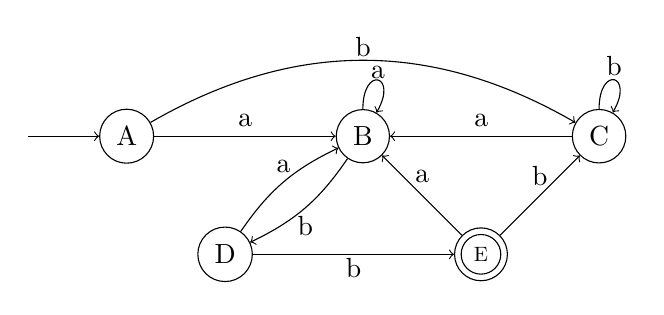
\begin{tikzpicture}
	\begin{pgfonlayer}{nodelayer}
		\node [style=new style] (0) at (-3, 0) {A};
		\node [style=new style] (1) at (0, 0) {B};
		\node [style=new style] (2) at (3, 0) {C};
		\node [style=new style] (3) at (-1.75, -1.5) {D};
		\node [style=new style] (4) at (1.5, -1.5) {E};
		\node [style=none] (5) at (-4.25, 0) {};
		\node [style=new style 0] (6) at (1.5, -1.5) {};
		\node [style=new style 0] (7) at (1.5, -1.5) {E};
	\end{pgfonlayer}
	\begin{pgfonlayer}{edgelayer}
		\draw [style=new edge style 0] (0) to node [above=0pt] {a} (1);
		\draw [style=new edge style 0] (2) to node [above=0pt] {a} (1);
		\draw [style=new edge style 0] (4) to node [above=0pt] {b} (2);
		\draw [style=new edge style 0, in=60, out=90, loop] (1) to node [above=-3pt] {a} ();
		\draw [style=new edge style 0, bend left] (0) to node [above=-2pt] {b} (2);
		\draw [style=new edge style 0, bend left=15] (3) to node [above=0pt] {a} (1);
		\draw [style=new edge style 0, bend left=15] (1) to node [above=-13.6pt] {b} (3);
		\draw [style=new edge style 0] (4) to node [above=1pt] {a} (1);
		\draw [style=new edge style 0, in=180, out=0] (3) to node [above=-12pt] {b} (4);
		\draw [style=new edge style 0] (5.center) to (0);
		\draw [style=new edge style 0, in=60, out=90, loop] (2) to node [above=-2pt] {b} ();
	\end{pgfonlayer}
\end{tikzpicture}
\end{center}
 14. Construct a regular grammar for the RE, L = (a + b)*(aa + bb)(a + b)*.
 \hspace*{0.5cm}	  		 \textit{\textbf{Solution:}} The NFA for the RE is
\begin{center}
    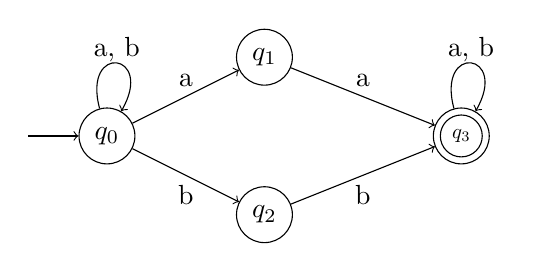
\begin{tikzpicture}
	\begin{pgfonlayer}{nodelayer}
		\node [style=new style] (0) at (-2, 0) {$q_0$};
		\node [style=new style] (1) at (2.5, 0) {$q_3$};
		\node [style=new style] (2) at (0, -1) {$q_2$};
		\node [style=new style] (3) at (0, 1) {$q_1$};
		\node [style=new style 0] (4) at (2.5, 0) {$q_3$};
		\node [style=none] (5) at (-3, 0) {};
	\end{pgfonlayer}
	\begin{pgfonlayer}{edgelayer}
		\draw [style=new edge style 0] (5.center) to (0);
		\draw [style=new edge style 0] (0) to node [above=0pt] {a} (3);
		\draw [style=new edge style 0] (0) to node [below=0pt] {b} (2);
		\draw [style=new edge style 0, in=60, out=105, loop] (0) to node [above=-3pt] {a, b} ();
		\draw [style=new edge style 0, in=60, out=105, loop] (1) to node [above=-3pt] {a, b} ();
		\draw [style=new edge style 0] (3) to node [above=0pt] {a} (1);
		\draw [style=new edge style 0] (2) to node [below=0pt] {b} (1);
	\end{pgfonlayer}
\end{tikzpicture}
\end{center}
There are four states in the FA. So, in the regular grammar, there are four non-terminals.
 Let us take them as A (for q\textsubscript{0}), B (for q\textsubscript{1}), C (for q\textsubscript{2}), and D (for q\textsubscript{3}).\\Now, we have to construct the production rules of the grammar.\\For the state q\textsubscript{0}, the production rules are\\ \hspace*{3cm} A → aA, A → bA, A → aB, A → bC.\\For the state q\textsubscript{1}, the production rules are\\ \hspace*{3cm} B → aD, B → a (as D is the final state).\\ For the state q\textsubscript{2}, the production rules are\\ \hspace*{3cm} C → b D, C → b (as D is the final state).\\For the state q\textsubscript{3}, the production rules are\\ \hspace*{3cm} D → aD, D → bD, D → a/ b.\\The grammar = \{V\textsubscript{N}, Σ, P, S\}\\ \hspace*{3cm}V\textsubscript{N} = \{A, B, C, D\} Σ = \{a, b\}\\
 \hspace*{3cm}P : A → aA/bA/aB/bC\\
 \hspace*{3cm}B → aD/a\\
 \hspace*{3cm}C → bD/b\\
 \hspace*{3cm}D → aD/bD/a/b.\\ \newpage
 \hspace*{-1.2cm} 15. Consider the given FA and construct the smallest DFA which accepts the same language. Draw an
RE and the grammar that generates it. \hspace*{1cm}[UPTU 2002]
\begin{center}
    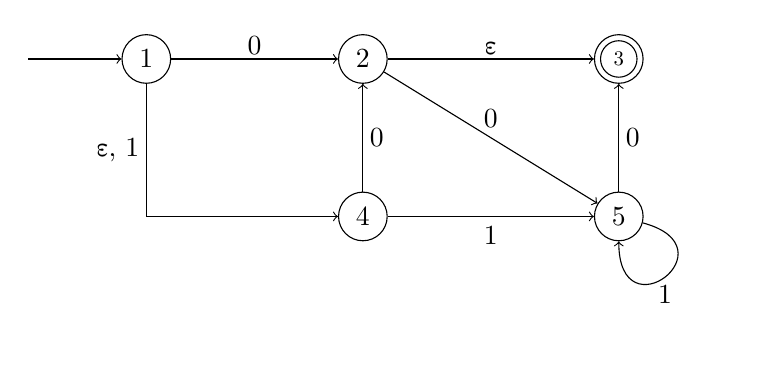
\begin{tikzpicture}
	\begin{pgfonlayer}{nodelayer}
		\node [style=new style] (0) at (-2.75, 3) {1};
		\node [style=new style] (1) at (0, 3) {2};
		\node [style=new style] (2) at (3.25, 3) {3};
		\node [style=new style] (3) at (0, 1) {4};
		\node [style=new style] (4) at (3.25, 1) {5};
		\node [style=none] (5) at (-2.75, 1) {};
		\node [style=none] (6) at (-4.25, 3) {};
		\node [style=new style 0] (7) at (3.25, 3) {3};
	\end{pgfonlayer}
	\begin{pgfonlayer}{edgelayer}
		\draw (0) to node [left=-1pt] {ε, 1} (5.center);
		\draw [style=new edge style 0] (5.center) to (3);
		\draw [style=new edge style 0] (0) to node [above=-2pt] {0} (1);
		\draw [style=new edge style 0] (3) to node [right=-1pt] {0} (1);
		\draw [style=new edge style 0] (1) to node [above=-2pt] {ε} (2);
		\draw [style=new edge style 0] (3) to node [below=0pt] {1} (4);
		\draw [style=new edge style 0] (4) to node [right=-1pt] {0} (2);
		\draw [style=new edge style 0, in=-90, out=-15, loop] (4) to node [above=-13pt] {1} ();
		\draw [style=new edge style 0] (1) to node [above=0pt] {0} (4);
		\draw [style=new edge style 0] (6.center) to (0);
	\end{pgfonlayer}
\end{tikzpicture}
\end{center}
 \textit{\textbf{Solution:}} This problem can be solved by the $\epsilon$-closure method.\\$\epsilon$-closure(1) = \{1, 4\} \hspace*{1cm} $\epsilon$-closure(3) = \{3\} \hspace*{1cm} $\epsilon$-closure(5) = \{5\} \\
 $\epsilon$-closure(2) = \{2, 3\} \hspace*{1cm} $\epsilon$-closure(4) = \{4\} \\As 1 is the beginning state,start with $\epsilon$-closure(1)=\{1,4\}.Let us rename it as A.
 A is still unmarked.\\Then, construct a δ' function for the new unmarked state A for inputs 0 and 1.\\
 δ'(A, 0) = $\epsilon$-closure(δ (A, 0))\hspace*{2cm}δ'(A, 1) = $\epsilon$-closure(δ (A, 1))\\
\hspace*{1.2cm} = $\epsilon$-closure (δ ((1,4), 0))\hspace*{2.6cm} = $\epsilon$-closure (δ ((1, 4), 1))\\
\hspace*{1.2cm} = $\epsilon$-closure (2, 2)\hspace*{3.7cm} = $\epsilon$-closure (4, 5)\\
\hspace*{1.2cm} = \{2, 3\}\hspace*{3.3cm} = $\epsilon$-closure (4) $\cup$ $\epsilon$-closure (5) = \{4, 5\}\\
It is a new state. Mark it as B.\hspace*{2.5cm}It is a new state. Mark it as C.\\
δ'(B, 0) = $\epsilon$-closure(δ (B, 0))\hspace*{2cm}δ'(B, 1) = $\epsilon$-closure(δ (B, 1))\\
 \hspace*{1.3cm}= $\epsilon$-closure (δ ((2, 3), 0))\hspace*{2.6cm}= $\epsilon$-closure (δ ((2, 3), 1))\\
 \hspace*{1.3cm}= $\epsilon$-closure (5)\hspace*{4.2cm}= $\epsilon$-closure ()\\
 \hspace*{1.3cm}= \{5\}\hspace*{5.9cm} = $\emptyset$\\
It is a new state. Mark it as D.\\
δ'(C, 0) = $\epsilon$-closure(δ (C, 0))\hspace*{2cm}δ'(C, 1) = $\epsilon$-closure(δ (C, 1))\\
 \hspace*{1.3cm}= $\epsilon$-closure (δ ((4, 5), 0))\hspace*{2.5cm} = $\epsilon$-closure (δ ((4, 5), 1))\\
 \hspace*{1.3cm}= $\epsilon$-closure (2, 3)\hspace*{3.7cm} = $\epsilon$-closure (5)\\
 \hspace*{1.3cm}= B\hspace*{5.8cm} = \{5\} = D\\
δ'(D, 0) = $\epsilon$-closure(δ (D, 0)) \hspace*{1.8cm}δ'(D, 1) = $\epsilon$-closure(δ (D, 1))\\
 \hspace*{1.2cm} = $\epsilon$-closure (δ ((5), 0)) \hspace*{2.8cm}= $\epsilon$-closure (δ (5), 1)\\
 \hspace*{1.2cm} = $\epsilon$-closure (3) \hspace*{4cm}= $\epsilon$-closure (5)\\
 \hspace*{1.2cm} = \{3\} \hspace*{5.8cm}= \{5\} = D\\
It is a new state. Mark it as E.\\
 δ'(E, 0) = $\epsilon$-closure(δ (E, 0)) \hspace*{1.8cm}δ'(E, 1) = $\epsilon$-closure(δ (E, 1))\\
 \hspace*{1.2cm} = $\epsilon$-closure (δ (3), 0) \hspace*{3cm}= $\epsilon$-closure (δ (5), 1)\\
 \hspace*{1.2cm} = $\emptyset$ \hspace*{5.7cm}= $\epsilon$-closure (5)\\
 \hspace*{7.7cm}= \{5\} = D\\
 The beginning state is A, and the final state is E.\newpage
 The transitional diagram of the DFA is
 \begin{center}
      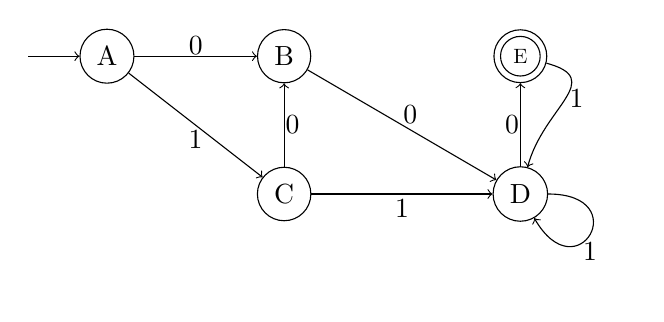
\begin{tikzpicture}
	\begin{pgfonlayer}{nodelayer}
		\node [style=new style] (0) at (0, 1.25) {B};
		\node [style=new style] (1) at (0, -0.5) {C};
		\node [style=new style] (2) at (-2.25, 1.25) {A};
		\node [style=new style] (3) at (3, -0.5) {D};
		\node [style=none] (4) at (-3.25, 1.25) {};
		\node [style=new style] (5) at (3, 1.25) {E};
		\node [style=new style 0] (6) at (3, 1.25) {E};
	\end{pgfonlayer}
	\begin{pgfonlayer}{edgelayer}
		\draw [style=new edge style 0] (4.center) to (2);
		\draw [style=new edge style 0] (2) to node [above=-3pt] {0} (0);
		\draw [style=new edge style 0] (2) to node [above=-12pt] {1} (1);
		\draw [style=new edge style 0] (1) to node [right=-3pt] {0} (0);
		\draw [style=new edge style 0] (1) to node [above=-12pt] {1} (3);
		\draw [style=new edge style 0] (0) to node [above right=-3pt] {0} (3);
		\draw [style=new edge style 0, in=-60, out=0, loop] (3) to node [above=-13pt] {1} ();
		\draw [style=new edge style 0] (3) to node [left=-3pt] {0} (5);
		\draw [style=new edge style 0, in=75, out=-15, looseness=1.50] (5) to node [right=-2pt] {1} (3);
	\end{pgfonlayer}
\end{tikzpicture}
 \end{center}
 The RE is constructed using the Arden’s theorem.\\
 \hspace*{5.1cm}A = $\land$\\
\hspace*{5cm} B = 0A + 0C\\
\hspace*{5cm} C = 1A\\
\hspace*{5cm} D = 0B + 1C + 1D + 1E\\
\hspace*{5cm} E = 0D\\
Replacing A in B and C, we get\\
\hspace*{5cm}B = 0 + 0C\\
\hspace*{5cm}C = 1.\\
Replacing C in B, we get B = 0 + 01.\\
Replacing the new value of B, C, and E in D, we get\\
\hspace*{5cm}BD = 0(0 + 01) + 11 + 1D + 10D\\
\hspace*{5cm}B= 0(0 + 01) + 11 + D(1 + 10).\\
It is in the format of R = Q + RP, where Q = (0 + (0 + 01) +11),P=(1 + 10).\\
 The solution is R = QP*.\\
 \hspace*{5cm}D = (0 + (0 + 01) + 11) (1 + 10)*\\
 Replacing the value of D in E, we get E = 0(0 + (0 + 01) + 11) (1 + 10)*.\\
 As E is the final state, the RE accepted by the FA is\\
\hspace*{5cm}0(0 + (0 + 01) + 11) (1 + 10)*.\\
The regular grammar is constructed as follows taking each state into account.\\
 There are fi ve states in the FA. So, in the regular grammar, there are fi ve non-terminals.\\
 Let us take them as A, B, C, D, and E according to the name of the states.\\
 Now we have to construct the production rules of the grammar.\\
 For the state A, the production rules are\\
 \hspace*{5cm}A → 0B, A → 1C.\\
 For the state B, the production rules are\\
 \hspace*{5cm}B → 0D \newpage
 
 
\hspace*{-0.6cm} For the state C, the production rules are\\
\hspace*{5cm} C → 0B C → 1D.\\
 For the state D, the production rules are\\
\hspace*{5cm} D → 1D D → 0E D → 0.\\
 For the state E, the production rules are\\
\hspace*{5cm} E → 1D.\\
\hspace*{-0.6cm}16. Find the RE recognized by the finite state automaton of the following figure. [GATE 1994]
\begin{center}
    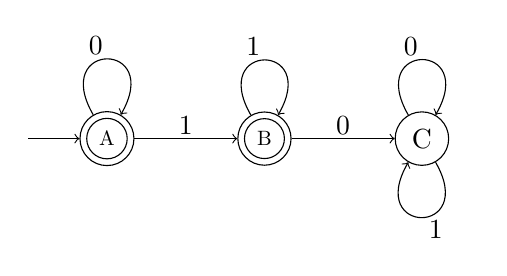
\begin{tikzpicture}
	\begin{pgfonlayer}{nodelayer}
		\node [style=new style] (0) at (-2, 0) {A};
		\node [style=new style] (1) at (0, 0) {B};
		\node [style=new style] (2) at (2, 0) {C};
		\node [style=none] (3) at (-3, 0) {};
		\node [style=new style 0] (4) at (-2, 0) {A};
		\node [style=new style 0] (5) at (0, 0) {B};
	\end{pgfonlayer}
	\begin{pgfonlayer}{edgelayer}
		\draw [style=new edge style 0] (0) to node [above=-2pt] {1} (1);
		\draw [style=new edge style 0] (1) to node [above=-2pt] {0} (2);
		\draw [style=new edge style 0] (3.center) to (0);
		\draw [style=new edge style 0, in=-120, out=-60, loop] (2) to node [above left=-11pt] {1} ();
		\draw [style=new edge style 0, in=60, out=120, loop] (2) to node [above left=-2pt] {0} ();
		\draw [style=new edge style 0, in=60, out=120, loop] (0) to node [above left=-2pt] {0} ();
		\draw [style=new edge style 0, in=60, out=120, loop] (1) to node [above left=-2pt] {1} ();
	\end{pgfonlayer}
\end{tikzpicture}
\end{center}
\textit{\textbf{Solution:}} The equation for the FA is\\
\hspace*{5cm} A = 0A + $\land$ \hspace*{4.5cm}(1)\\
\hspace*{5cm} B = 1A + 1B \hspace*{4.3cm}(2)\\
\hspace*{5cm} C = 0B + 0C + 1C \hspace*{3.5cm}(3)\\
Solving the equation (1) using the Arden’s theorem, we get A = $\land$0* = 0*.\\
 Putting the value of A in equation (2), we get\\
\hspace*{5cm} B = 10* + 1B.\\
 Using the Arden’s theorem, we get\\
\hspace*{5cm} B = 10*1*.\\
 Both A and B are final states, and thus the string accepted by the FA is\\
\hspace*{5cm} 0* + 10*1*\\
\hspace*{5cm}= 0* ($\land$ + 11*) = 0*1* (as $\land$ + RR* = R*).
\begin{figure}[!ht]
\centering
\includegraphics[scale=0.6]{288.png}
\end{figure}\\
\small
1. The machine format of regular expression is:\\ \hspace*{0.1cm}a) Finite automata \hspace*{0.1cm}b) Push down automata \hspace*{0.2cm}c) Turing machine\hspace*{0.5cm}d) All of the above\\
 2. The regular expression is accepted by:\\ a) Finite automata\hspace*{0.5cm}b) Push down automata\hspace*{0.5cm}c) Turing machine\hspace*{0.5cm}d) All of the above\\
3. The language of all words with at least 2 a’s can be described by the regular expression:\\ a) (ab)*a\hspace*{0.5cm}b) (a + b)*ab*a(a + b)*\hspace*{0.5cm} c) b*ab*a(a + b)*\hspace*{0.5cm}d) All of the above\\
 4. The set of all strings of \{0, 1\} having exactly two 0’s is:\\ 
 a) 1*01*01*\hspace*{0.5cm} b) \{0 + 1)*1\hspace*{0.5cm} c) \{11 + 0\}*\hspace*{0.5cm}d) \{00 + 11\}*
 \end{document}
